The \textbf{ion species} is defined by the chemical name of an atom (e.g.,
\texttt{He} or \texttt{B}) or of a molecule (e.g., \texttt{BF2} for a
boron difluoride molecule). In case of a molecule, the \textbf{ion energy} is
considered the kinetic energy of the molecule, and the individual atom energies are
derived based on the atom masses. Each atom of the molecule is
implanted one after another. For instance, if the ion is \texttt{BF2}, then one
B atom is followed by two F atoms. Currently, the initial conditions of each 
molecule atom are treated as independent from each other, i.e., any property 
defined by a statistical distribution uses different random numbers for each 
molecule atom. This approximation is not expected to make a difference in
most if not all cases. It is also possible to specify the \textbf{mass} of the
atoms in order to distinguish isotopes.

The \textbf{starting points} of the ion trajectories are determined in several
steps. First, a reference point is defined. Its coordinates are chosen uniformly
distributed in an axis-parallel brick. Degenerate forms of the brick, a
rectangle, a line, or a single position are also possible. If a beam profile
with a nonzero full-width-at-half-maximum is specified, this reference point is
moved in the plane perpendicular to the beam direction by a Gaussian distributed
displacement. If a crystalline region is specified and an external beam is
chosen, the reference point is additionally moved by a vector between a corner
of the crystal unit cell to a random point inside the cell. If at least one
crystalline region is specified and the ions are chosen to start inside the
target, the reference point is additionally moved to the nearest lattice site. 
Finally, in case of an external beam and if the reference point is inside the
target, the starting point is obtained by projecting the reference point to the
surface. This is done along the ion direction to a position which is a
distance equal to the maximum impact parameter outside the target, where the
ion, when coming from infinity along a straight line, first hits the target.
Otherwise, the ion starts at the reference point. 

\begin{figure}[htbp]
\centering
\noindent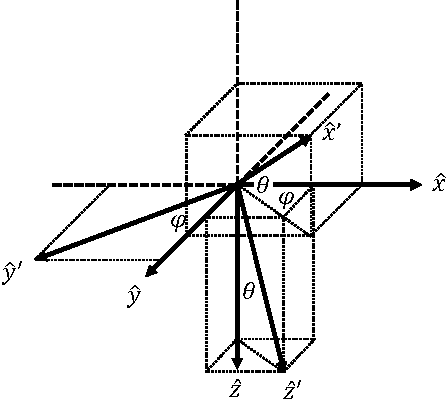
\includegraphics[scale=1.0]{coordinate_systems-crop.pdf}
\caption{Definition of the beam coordinate system $(\hat{x}', \hat{y}',
\hat{z}')$ and the target coordinate system $(\hat{x}, \hat{y}, \hat{z})$ by
tilt angle $\theta$ and rotation angle $\varphi$.}
\label{fig:coord}
\end{figure}   
%
The \textbf{initial direction} of the ions is defined by a reference direction
and, optionally, an additional rotation due to beam  divergence.
The reference direction is defined by a tilt and a rotation angle relative to
the target coordinate system, see Fig.~\ref{fig:coord}. The tilt and rotation
angles may be specified, or the rotation angle may be chosen randomly for each
ion. Without beam divergence the initial directions of all ions coincide with
the reference direction $\hat{z}'$ (cf.\ Fig.~\ref{fig:coord}). Considering a
beam divergence means to randomly rotate the ion’s direction of motion on the
unit sphere from the beam direction in such a way that the probability per solid
angle follows a given distribution. Two beam divergence models may be chosen from:
isotropic within a maximum rotation angle and Gaussian with given standard
deviations in $\hat{x}'$ and $\hat{y}'$ direction.

\begin{figure}[htbp]
\centering
\noindent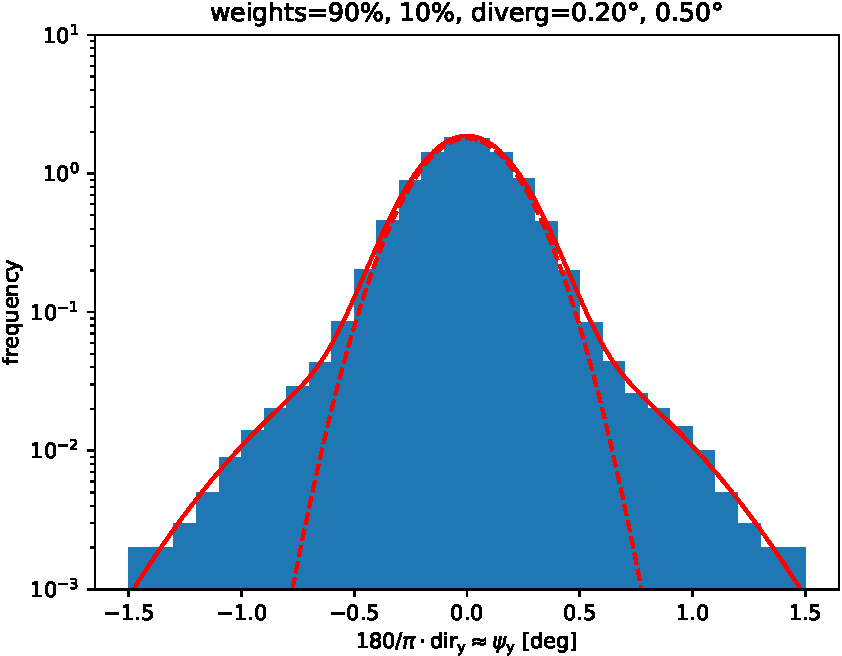
\includegraphics[scale=0.8]{diverg_y-crop.pdf}
\caption{Beam profile composed of two Gaussian functions (red line) and
histogram of angles \(\psi_\mathrm{y}\) generated by IMSIL.}
\label{fig:diverg}
\end{figure}  
%
More refined beam profiles or divergence distributions may be defined by
superposing partial beams using the \texttt{BEAM} index variable. An index
variable used on an input record specifies that the parameters on this record
apply to a particular object only, in this case to a partial beam. Each partial
beam may have a different beam profile and/or beam divergence. Ions are then
chosen with probabilities proportional to a specified beam weight from each of
the partial beams. An example for the superposition of two Gaussian beam
divergence distributions is shown in Fig.~\ref{fig:diverg}. Below is an excerpt
from an IMSIL input file that specifies the above beam profile: 
%
\begin{verbatim}
   &IONS NAME='B' ENERGY=5000 DOSE=1e13 TILT=0 MODDIV=2 NION=10000 /
   &IONS BEAM=1 WEIGHT=0.9 DIVERG=0.1,0.2 /
   &IONS BEAM=2 WEIGHT=0.1 DIVERG=0.2,0.5 /
\end{verbatim}
%
Note that parameters that are specified on the first line, which does not have
the \texttt{BEAM} index parameter, apply to both beams.

The \textbf{ion dose} may either be specified in ions per area in the $x$-$y$
plane (areal dose, units cm$^{-2}$), ions per length in $y$ direction (line
dose, units cm$^{-1}$), or ion count. The most natural choice among these
options depends on the dimensionality of the spatial histograms that are
computed: areal dose for 1-D, line dose for 2-D, and number doses for 3-D
histograms. However, other choices are possible, see Sections~\ref{s:his1d},
\ref{s:his2d}, and \ref{s:his3d}.

\begin{center}
\begin{tabular}{lll}
parameter \quad              & IMSIL name      & to be specified in record \\
\hline
internal starting point flag & \texttt{LIINIT}    & \texttt{\&IONS} \\
ion name                     & \texttt{NAME}      & \texttt{\&IONS} \\
energy                       & \texttt{ENERGY}    & \texttt{\&IONS} \\
atom mass                    & \texttt{MASS}      & \texttt{\&ATOMS} \\
reference starting point     & \texttt{XINIT}     & \texttt{\&IONS} \\
                             & \texttt{YINIT}     & \texttt{\&IONS} \\
                             & \texttt{ZINIT}     & \texttt{\&IONS} \\
beam FWHM                    & \texttt{FWHM}      & \texttt{\&IONS} \\
tilt angle                   & \texttt{TILT}      & \texttt{\&IONS} \\
rotation angle               & \texttt{ROTATE}    & \texttt{\&IONS} \\
random rotation flag         & \texttt{RANROT}    & \texttt{\&IONS} \\
beam divergence model        & \texttt{MODDIV}    & \texttt{\&IONS} \\
beam divergence              & \texttt{DIVERG}    & \texttt{\&IONS} \\
beam index variable          & \texttt{BEAM}      & \texttt{\&IONS} \\
beam weight                  & \texttt{WEIGHT}    & \texttt{\&IONS} \\
dose                         & \texttt{DOSE}      & \texttt{\&IONS} \\
dose units                   & \texttt{DOSEUNITS} & \texttt{\&IONS} \\
number of simulated ions     & \texttt{NION}      & \texttt{\&IONS} \\
\end{tabular}
\end{center}
